\documentclass{csse4400}

% \teachermodetrue

\usepackage{float}
\usepackage{languages}
\usepackage{changepage}

\title{Load Testing \& Bottlenecks}
\author{Brae Webb \& Richard Thomas}

\date{\week[practical]{9}}
\begin{document}

\maketitle

\begin{figure}[h]
    \centering
    
\includegraphics[width=0.8\textwidth]{images/bottleneck}
\end{figure}

\aside{
  Github Classroom links for this practical can be found on Edstem \url{https://edstem.org/au/courses/21491/discussion/2429006}
}

\warning{
  This practical \textbf{cannot} be completed on Windows.
  The Docker provider for Terraform encounters an error when creating an image on Windows.
  You will need to use WSL instead of the native Windows environment.
}


\section{This Week}
Our goal is to:
\begin{itemize}
  \item Introduce structured logging to TaskOverflow.
  \item Re-deploy TaskOverflow to AWS.
  \item Write k6 tests to ensure TaskOverflow can handle given scenarios.
  \item Uncover and fix bottlenecks in the TaskOverflow application using the logs.
\end{itemize}


\section{Watchtower}
In this course we have repeatedly claimed that there is value in monitoring and logging.
This week, we aim to prove it by using logging to help diagnose issues with a deployment of TaskOverflow.
For this task, we have integrated \link{Watchtower}{https://pypi.org/project/watchtower/} into the project.
Watchtower is a Python library that allows us to send logs to AWS CloudWatch,
allowing us to monitor an application's performance in real time.

Currently the project is configured to log API accesses made with Flask and to log database queries created by SQL Alchemy.
This results in an unstructured log stream as seen in Figure \ref{fig:cloud-logs}.

\begin{figure}[ht]
    \centering
    \begin{adjustwidth}{-7.5mm}{-7.5mm}
        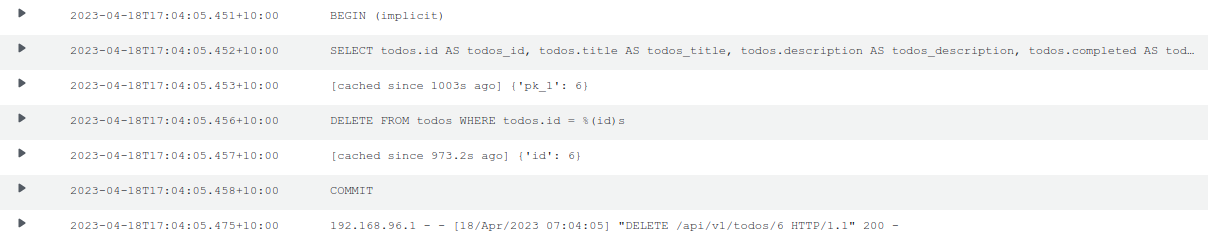
\includegraphics[width=0.95\paperwidth]{images/cloud-watch-log}
    \end{adjustwidth}
    \caption{An example of logs made to AWS CloudWatch for a DELETE request in the TaskOverflow API.}
    \label{fig:cloud-logs}
\end{figure}

\paragraph{Getting Started}
\begin{enumerate}
    \item Using the GitHub Classroom link for this practical, provided on edstem, create a repository to work within.
    \item Start your Learner Lab and copy the AWS Learner Lab credentials into a credentials file in the root of the repository.
\end{enumerate}

\paragraph{What's New}
We are returning to TaskOverflow roughly from the state at the end of the
\textit{Scaling Stateless Components} practical \cite{prac-week6}.
The following notable changes have been made:
\begin{itemize}
    \item \texttt{Watchtower} has been installed as a dependency.
    \item In \texttt{docker-compose.yml}, we mount the \texttt{credentials} file to \texttt{/root/.aws/credentials}.
        This allows local testing of \texttt{watchtower} to log to AWS CloudWatch.
    \item Logging has been introduced for Flask and SQL Alchemy.
\end{itemize}

Our first task will be to replicate the above logs in Figure \ref{fig:cloud-logs}.
Once you have copied \texttt{credentials} into the project root directory,
start docker compose with:
\bash{docker compose up}

\begin{code}[numbers=none]{}
app-1       |  * Serving Flask app 'todo'
app-1       |  * Debug mode: on
app-1       | INFO:werkzeug:WARNING: This is a development server. Do not use it in a production deployment. Use a production WSGI server instead.
app-1       |  * Running on all addresses (0.0.0.0)
app-1       |  * Running on http://127.0.0.1:6400
app-1       |  * Running on http://172.18.0.3:6400
app-1       | INFO:werkzeug:Press CTRL+C to quit
app-1       | INFO:werkzeug: * Restarting with stat
app-1       | INFO:botocore.credentials:Found credentials in shared credentials file: ~/.aws/credentials
app-1       | INFO:sqlalchemy.engine.Engine:select pg_catalog.version()
app-1       | INFO:sqlalchemy.engine.Engine:[raw sql] {}
app-1       | INFO:sqlalchemy.engine.Engine:select current_schema()
app-1       | INFO:sqlalchemy.engine.Engine:[raw sql] {}
app-1       | INFO:sqlalchemy.engine.Engine:show standard_conforming_strings
app-1       | INFO:sqlalchemy.engine.Engine:[raw sql] {}
app-1       | INFO:sqlalchemy.engine.Engine:BEGIN (implicit)
app-1       | INFO:sqlalchemy.engine.Engine:SELECT pg_catalog.pg_class.relname
app-1       | FROM pg_catalog.pg_class JOIN pg_catalog.pg_namespace ON pg_catalog.pg_namespace.oid = pg_catalog.pg_class.relnamespace
app-1       | WHERE pg_catalog.pg_class.relname = %(table_name)s::VARCHAR AND pg_catalog.pg_class.relkind = ANY (ARRAY[%(param_1)s::VARCHAR, %(param_2)s::VARCHAR, %(param_3)s::VARCHAR, %(param_4)s::VARCHAR, %(param_5)s::VARCHAR]) AND pg_catalog.pg_table_is_visible(pg_catalog.pg_class.oid) AND pg_catalog.pg_namespace.nspname != %(nspname_1)s::VARCHAR
app-1       | INFO:sqlalchemy.engine.Engine:[generated in 0.00015s] {'table_name': 'todos', 'param_1': 'r', 'param_2': 'p', 'param_3': 'f', 'param_4': 'v', 'param_5': 'm', 'nspname_1': 'pg_catalog'}
app-1       | INFO:sqlalchemy.engine.Engine:COMMIT
app-1       | WARNING:werkzeug: * Debugger is active!
app-1       | INFO:werkzeug: * Debugger PIN: 123-456-789
\end{code}

You should see logs similar to the above.
Notice that information about Flask is prefixed with \texttt{INFO:werkzeug} and information about SQL Alchemy is prefixed with \texttt{INFO:sqlalchemy.engine.Engine}.
These prefixes indicate into which stream the logs are put.

Open the AWS CloudWatch console and go to \texttt{Logs > Log groups} on the side panel.
You should see a log group called \texttt{taskoverflow}.
If you click on that group you will see log streams associated with \texttt{INFO:werkzeug}
and \texttt{INFO:sqlalchemy.engine.Engine}.

\begin{center}
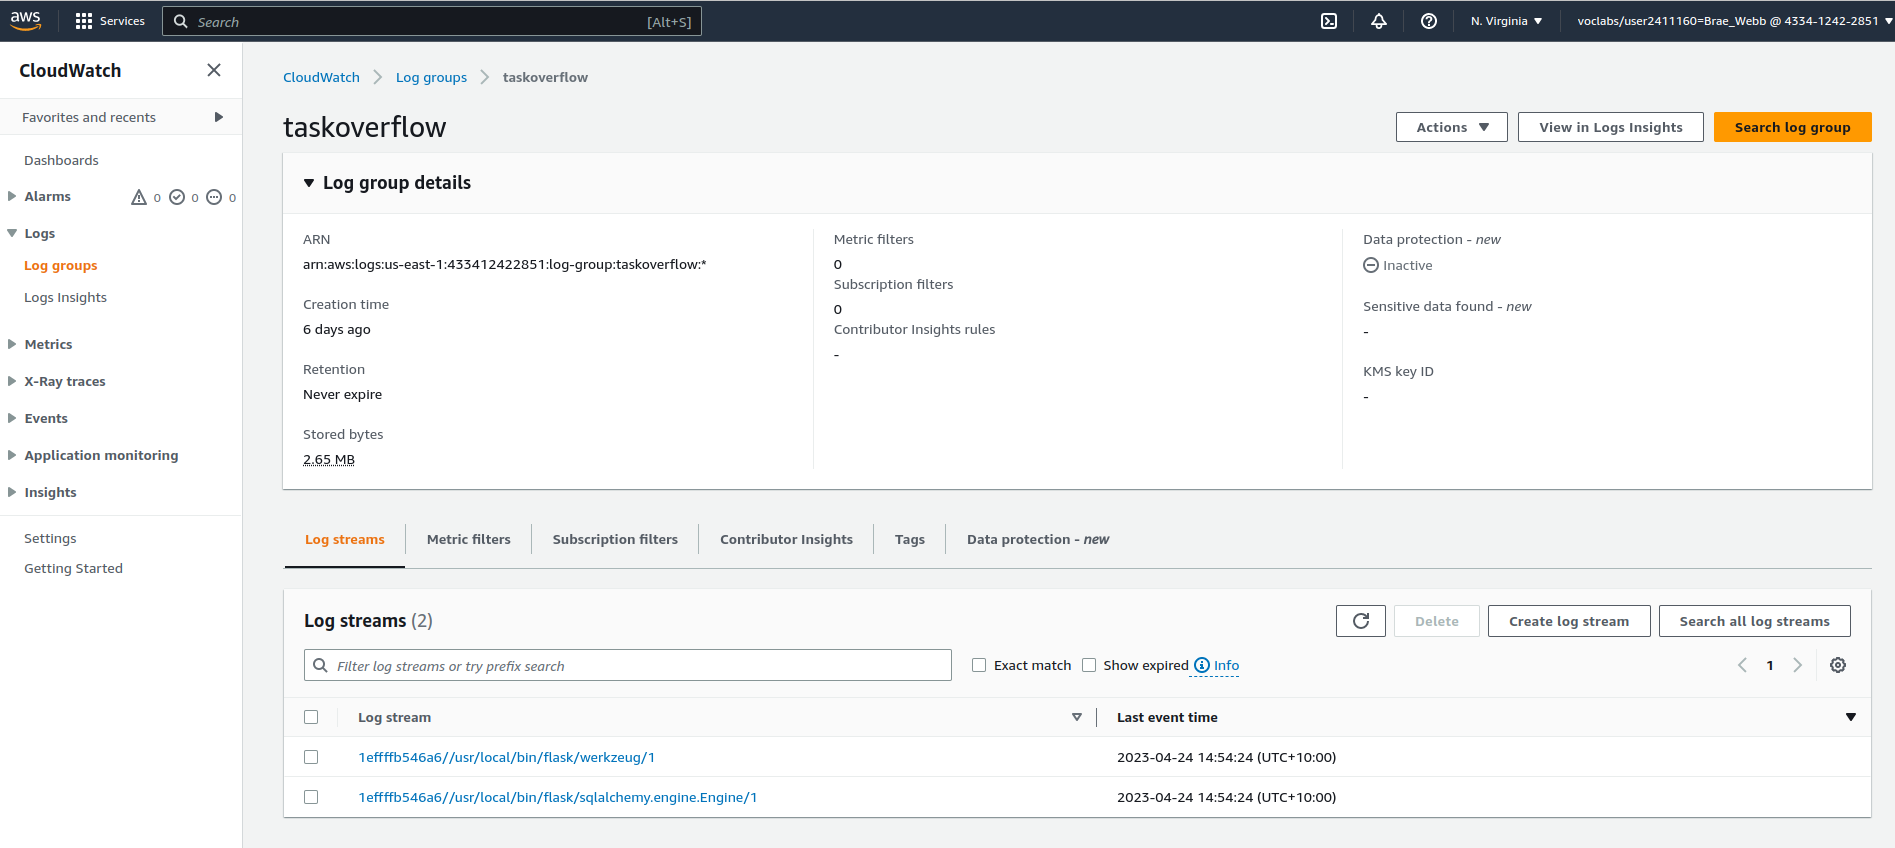
\includegraphics[width=\textwidth]{images/log-group}
\end{center}

\subsection{Structured Logging}

Our first task will be to convert the current logging into a structured logging format.
As we saw in logging lecture \cite{logging-slides}, structured logging can be as simple as logging a JSON object.
This allows logging services to quickly filter through logs based on criteria selected from the object's fields.

In \texttt{todo/\_\_init\_\_.py} we have the following code within the \texttt{create\_app} function.
This code configures watchtower to log to AWS CloudWatch.
%
\begin{code}[language=python,numbers=none]{todo/\_\_init\_\_.py}
def create_app(config_overrides=None): 
    ...
    handler = watchtower.CloudWatchLogHandler(
        log_group_name="taskoverflow",
        boto3_client=boto3.client("logs", region_name="us-east-1")
    )
    app.logger.addHandler(handler)
    ...
\end{code}

We want to wrap all our logs in JSON objects and inject metadata into these objects.
This makes it easier to search the logs.
To do this, we will create a custom log formatter that is a subclass of \\
\texttt{watchtower.CloudWatchLogFormatter}.
%
\begin{code}[language=python,numbers=none]{todo/\_\_init\_\_.py}
from flask import has_request_context, request
...

class StructuredFormatter(watchtower.CloudWatchLogFormatter):
    def format(self, record):
        record.msg = {
            'timestamp': record.created,
            'location': record.name,
            'message': record.msg,
        }
        if has_request_context():
            record.msg['request_id'] = request.environ.get('REQUEST_ID')
            record.msg['url'] = request.environ.get('PATH_INFO')
            record.msg['method'] = request.environ.get('REQUEST_METHOD')
        return super().format(record)

def create_app(config_overrides=None): 
    ...
    handler = ...
    handler.setFormatter(StructuredFormatter())
    ...
\end{code}

These are just some metadata fields we might want to add to our logging.
We may also consider \texttt{socket.gethostname()} to identify the instance handling a request,
or other helpful information.

\subsection{Correlation IDs}

Correlation IDs are a mechanism to help understand the path of a request, event, message, etc. through a system.
When logging it is often helpful to be able to trace the execution of a particular request.

For our system we will generate a new random identifier for each incoming request.
This identifier will be included as part of the logging metadata.
For a system with multiple API endpoints requests will often come with an established REQUEST\_ID header.
%
\begin{code}[language=python,numbers=none]{todo/\_\_init\_\_.py}
import uuid
...

def create_app(config_overrides=None): 
    ...
    requests = logging.getLogger("requests")
    requests.addHandler(handler)

    @app.before_request
    def before_request():
        request.environ['REQUEST_ID'] = str(uuid.uuid4())
        requests.info("Request started")

    @app.after_request
    def after_request(response):
        requests.info("Request finished")
        return response
    ...
\end{code}

The code above in \texttt{create\_app} will generate a unique identifier for each incoming request.
It will also log when a request starts being processed and when it finishes processing.

\subsection{Verify and Refine}
Ensure that the above modifications are working as expected by returning to the AWS CloudWatch logs.
Launch the service locally and make some API requests.

You should now be able to go to the \texttt{Log Insights} interface from the sidebar.
This interface allows you to query structured logging data.
Try the following query to ensure that your logs seem sensible.
%
\begin{code}[numbers=none]{}
fields request_id, url, method, @timestamp, message.message, @message, @method
| filter not isempty(request_id)
| limit 400
\end{code}

Take the time to refine your logging now to produce logs that are easy to search through
and understand the trace of your API requests.


\section{Load Testing}

We will now generate some load on our API using \texttt{k6} and see how it performs.
We briefly saw \texttt{k6} at the end of the \textit{Scaling Stateless Components} practical \cite{prac-week6}.
To review, \texttt{k6} is a load testing tool that is written in Go but provides an interface using a subset of JavaScript.

It will help us to generate a large number of concurrent API requests.
If you have not already done so, install \texttt{k6} from:
\url{https://k6.io/docs/get-started/installation/}

\subsection{Scenario}
We want to simulate the following scenario using our testing framework.

\paragraph{Indecisive planners and studious reviewers}
Our TaskOverflow application is being used at a point in semester where most students have already setup their tasks.
These students are routinely visiting the website and listing the tasks they have yet to complete.
At the same time, there are 40 very indecisive students who,
quite late in semester,
are trying to setup their tasks for the rest of semester.
They continually create a task,
realise that they have mis-typed,
delete the task,
and start over.

As the tasks are shared globally amongst all students,
the indecisive planners are altering the list of task seen by the organised students.

\subsection{Setup}
To get started,
we will create a file called \texttt{planners-and-studiers.js}.
Most \texttt{k6} tests start with the following imports.
%
\begin{code}[language=JavaScript,numbers=none]{planners-and-studiers.js}
import http from "k6/http";
import { check, sleep } from "k6";

const ENDPOINT = __ENV.ENDPOINT;
\end{code}

\begin{itemize}
    \item \texttt{http} holds the methods used to make HTTP requests,
    \item \texttt{check} allows us to assert the state of HTTP responses, and
    \item \texttt{sleep} gives us the ability to put a simulated user to sleep rather than continuously spamming the service with requests.
\end{itemize}

The ENDPOINT line retrieves the endpoint URL from the ENDPOINT environment variable.

\subsection{User Simulation}

The behaviour of our users will be defined by an exported JavaScript function.
Our studying student will be listing out all of the tasks they have left to complete by using the
\texttt{/api/v1/todos} endpoint.
%
\begin{code}[language=JavaScript,numbers=none]{planners-and-studiers.js}
export function studyingStudent() {
    let url = ENDPOINT + '/api/v1/todos';

    // What tasks do I have left to work on?
    let request = http.get(url);

    check(request, {
        'is status 200': (r) => r.status === 200,
    });
    
    // Alright I'll go work on my next task for around 2 minutes
    sleep(120);
}
\end{code}

Of course,
this test is very basic as it only ensures the response code is 200.
There is no guarantee that the returned data is sensible.

\info{
If you would like a challenge,
you can use the \texttt{randomIntBetween} function to have the studier occasionally tick off tasks.

\url{https://k6.io/docs/javascript-api/jslib/utils/randomintbetween/}
}

Next we need to simulate our indecisive students.
For them, we will need to make a POST request to the \texttt{/api/v1/todos} endpoint to create a task.
Then we will need to use the ID given by the POST response to DELETE the mis-typed task.
%
\begin{code}[language=JavaScript,numbers=none]{planners-and-studiers.js}
export function indecisivePlanner() {
    let url = ENDPOINT + '/api/v1/todos';

    // I need to work on the CSSE6400 Cloud Assignment!
    const payload = JSON.stringify({
        "title": "CSSE6400 Clout Assignment",
        "completed": false,
        "description": "",
        "deadline_at": "2025-09-05T15:00:00",
    });

    const params = {
        headers: {
            'Content-Type': 'application/json',
        },
    };

    let request = http.post(url, payload, params);
    check(request, {
        'is status 200': (r) => r.status === 200,
    });

    sleep(10);

    // Oh no! Not the Clout assignment, the Cloud assignment!
    const wrongId = request.id;

    request = http.del('${url}/${wrongId}');

    check(request, {
        'is status 200': (r) => r.status === 200,
    });

    // I'll come back to it later :(
    sleep(10);
}
\end{code}

\subsection{Configure Behaviour}

We have now outlined how our user agents will interact with our API.
We can use the \texttt{options} to configure how these interactions occur over time.
To prevent overloading the API immediately,
and allow any auto-scaling behaviour to be triggered,
we will slowly increase the amount of studiers.
We will have a consistent amount of planners, 20,
who will perform a total of 200 corrections over the test.
%
\begin{code}[language=JavaScript,numbers=none]{planners-and-studiers.js}
export const options = {
    scenarios: {
        studier: {
            exec: 'studyingStudent',
            executor: "ramping-vus",
            stages: [
                { duration: "1m", target: 1500 },
                { duration: "3m", target: 7500 },
                { duration: "2m", target: 0 },
            ],
        },
        planner: {
            exec: 'indecisivePlanner',
            executor: "shared-iterations",
            vus: 20,
            iterations: 200,
        },
    },
};
\end{code}

\subsection{Running the Tests}

Now we have a completed load test.
Deploy the service to AWS:

\bash{terraform init}
\bash{terraform apply}

Once the deployment is finished,
you should be given a URL where the endpoint is deployed.
Use that endpoint to set the \texttt{ENDPOINT} environment variable and run the tests.
%
\begin{code}[language=bash,numbers=none]{}
> export ENDPOINT=...
> k6 run planners-and-studiers.js
\end{code}

These tests should take about 10 minutes to run.
You should see that most of the tests pass but that there will be a few failures throughout,
as seen below.
%
\begin{code}[language=bash,numbers=none]{}
WARN[0152] Request Failed                                error="Get \"http://taskoverflow-451078826.us-east-1.elb.amazonaws.com/api/v1/todos\": request timeout"
WARN[0183] Request Failed                                error="Get \"http://taskoverflow-451078826.us-east-1.elb.amazonaws.com/api/v1/todos\": request timeout"
WARN[0239] Request Failed                                error="Get \"http://taskoverflow-451078826.us-east-1.elb.amazonaws.com/api/v1/todos\": request timeout"
WARN[0241] Request Failed                                error="Delete \"$%7Burl%7D/$%7BwrongId%7D\": unsupported protocol scheme \"\""
WARN[0272] Request Failed                                error="Get \"http://taskoverflow-451078826.us-east-1.elb.amazonaws.com/api/v1/todos\": request timeout"
WARN[0330] Request Failed                                error="Get \"http://taskoverflow-451078826.us-east-1.elb.amazonaws.com/api/v1/todos\": request timeout"
WARN[0339] Request Failed                                error="Get \"http://taskoverflow-451078826.us-east-1.elb.amazonaws.com/api/v1/todos\": request timeout"
WARN[0371] Request Failed                                error="Get \"http://taskoverflow-451078826.us-east-1.elb.amazonaws.com/api/v1/todos\": request timeout"
WARN[0412] Request Failed                                error="Get \"http://taskoverflow-451078826.us-east-1.elb.amazonaws.com/api/v1/todos\": request timeout"

    TOTAL RESULTS

    checks_total...................: 16498  32.852733/s
    checks_succeeded...............: 92.47% 15257 out of 16498
    checks_failed..................: 7.52%  1241 out of 16498

      is status 200
         92% -   15257 /   1241

    HTTP
    http_req_duration...........................................: avg=14.05s min=0s       med=3.82s max=59.99s p(90)=49.14s p(95)=51.71s
      { expected_response:true }................................: avg=14.32s min=227.64ms med=3.81s max=59.72s p(90)=49.3s  p(95)=51.7s
    http_req_failed.............................................: 5.13%  847 out of 16498
    http_reqs...................................................: 16498  32.852733/s

    EXECUTION
    iteration_duration..........................................: avg=2m0s   min=20.22s   med=2m3s  max=2m38s  p(90)=2m10s  p(95)=2m20s
    iterations..................................................: 10422  20.753496/s
    vus.........................................................: 3      min=3            max=7520
    vus_max.....................................................: 7520   min=7520         max=7520

    NETWORK
    data_received...............................................: 1.5 GB 3.1 MB/s
    data_sent...................................................: 2.3 MB 4.5 kB/s




running (08m22.2s), 0000/7520 VUs, 10422 complete and 6329 interrupted iterations
planner   [======================================] 20 VUs         08m22.2s/10m0s  400/400 shared iters
studier   [======================================] 0000/7500 VUs  7m0s
\end{code}


\section{Debugging}

Now we can start to debug our service.
We desire to not only increase our 92\% pass rate to 100\%,
but also to increase the amount of studiers and planners.

\subsection{Tips}

\paragraph{Open TaskOverflow}
If you open TaskOverflow,
you should find it has been left in an unusual state after the tests.
See if you can find out from the logs how this occurred.

\paragraph{Follow an Interaction}
Use the correlation IDs that we have included to see where potential bottlenecks may be occurring.
You can introduce more fine-grained logs to identify where time is being spent.

\teacher{
Solutions are roughly:

1. Discover that DELETE /api/v1/todos/undefined is being requested from the logs.
Change 
    const wrongId = request.id;
to
    const wrongId = request.json().id;

2. Find that more tests are failing then there are timeouts.
Change expected HTTP status code for POST to 201.

3. Recognise that even with these fixes, the requests still timeout.
Upgrade the ECS task from 1 CPU / 2GB memory to maybe 4 CPU / 8GB memory.
}


\bibliographystyle{ieeetr}
\bibliography{books,ours}

\end{document}
